\documentclass[conference]{IEEEtran}
\usepackage{times}
\usepackage[T1]{fontenc}
\usepackage{cite}
\usepackage{amsmath,amssymb}
\usepackage{graphicx}
\usepackage{booktabs}
\usepackage{array}
\usepackage[hidelinks]{hyperref}
\usepackage{xcolor}
\graphicspath{{../figures/ieee/}}
\hyphenation{multi-plier gem5 micro-bench-mark}
\newcommand{\silu}{SiLU}
\newcommand{\ffour}{$f_4$}

\begin{document}

\title{Hardware--Software Co-Design of a Multiplier-Less SiLU Custom Instruction for RISC-V: In-Order versus Out-of-Order in gem5}

\author{\IEEEauthorblockN{Ayush Krishna}
\IEEEauthorblockA{School of Electronics Engineering\\Vellore Institute of Technology, Vellore, India\\ayush.krishna2025@vitstudent.ac.in}
\and
\IEEEauthorblockN{Vrinda Pandey}
\IEEEauthorblockA{School of Electronics Engineering\\Vellore Institute of Technology, Vellore, India\\vrinda.pandey2025@vitstudent.ac.in}
\and
\IEEEauthorblockN{Tanvee Chintala}
\IEEEauthorblockA{School of Electronics Engineering\\Vellore Institute of Technology, Vellore, India\\chintala.tanvee2025@student.ac.in}
\and
\IEEEauthorblockN{Chandni Srivastava}
\IEEEauthorblockA{School of Electronics Engineering\\Vellore Institute of Technology, Vellore, India\\chandni.srivastava2025@vitstudent.ac.in}
\and
\IEEEauthorblockN{Eswar Sesha Sai}
\IEEEauthorblockA{School of Electronics Engineering\\Vellore Institute of Technology, Vellore, India\\Eswar.sesha2025@vitstudent.ac.in}}

\maketitle

\begin{abstract}
The Sigmoid Linear Unit (SiLU) is the activation function of YOLOv8 and many other networks; without a hardware exponential it is computed by an expensive library call. This paper evaluates a published multiplier-free, six-segment piecewise-linear SiLU approximation as a RISC-V custom instruction. The approximation is implemented in Verilog, synthesised for an FPGA, and added to the gem5 simulator, where the functional-unit latency is derived from the synthesis delay by a script rather than entered by hand. The same binaries run on in-order and out-of-order cores, and instruction count, cycles per instruction, latency, pipelining, branch mispredictions, code placement and cache size are measured. The approximation is then substituted into YOLOv8n to measure accuracy and an Amdahl-bounded whole-network speedup. On an activation loop the instruction is 24$\times$ (in-order) and 36$\times$ (out-of-order) faster than a C library exponential, but only 2.4$\times$ and 3.7$\times$ faster than the same approximation in integer C. For a scalar-core network the gain is about 1.1$\times$ over the exponential and 1.01--1.02$\times$ over integer C, rising to 2.5--2.7$\times$ over the exponential only if multiply-accumulate work is 16$\times$ faster. Accuracy loss beyond fixed-point rounding is about 0.0015 mAP50--95 on a 128-image set.
\end{abstract}

\begin{IEEEkeywords}
Amdahl's law, custom instruction, gem5, hardware--software co-design, out-of-order execution, RISC-V, SiLU
\end{IEEEkeywords}

\section{Introduction}
Activation functions are a small part of a neural network's arithmetic but are awkward on simple processors: SiLU \cite{elfwing2018,ramachandran2017} needs an exponential and a division. A natural architectural reply is a custom instruction. Whether that pays off is a computer-architecture question, not a circuit question: it depends on how many instructions the baseline needs, on cycles per instruction (CPI) in the pipeline that executes it, on the clock period, and on what fraction of total run time the function occupies. This work therefore treats the instruction as an object to be evaluated with the quantitative tools of computer architecture --- the iron law, Amdahl's law, hazards, in-order versus out-of-order execution, and branch prediction --- rather than as a stand-alone circuit.

\textbf{Contributions.}
(1) A complete, scripted flow from RTL and timing report to a gem5 functional unit whose latency is computed (not hand-entered) from the synthesis delay and the target clock.
(2) A fair comparison of five code variants (loop only, C \texttt{expf}, integer approximation, 257-entry table, custom instruction) on two core models, across clocks and latencies, with branch, alignment, and cache controls.
(3) A model-level evaluation on YOLOv8n that separates accuracy from speed and bounds the speed benefit by Amdahl's law.
(4) An explicit statement of what these simulations cannot show.

\section{Background}
\subsection{The approximation}
Spagnolo, Perri and Corsonello \cite{spagnolo2025} propose piecewise-linear approximations of Swish (SiLU) that need only shifts and adds. We use their six-segment variant (``$f_4$'' in our code) in Q6.10 fixed point (16-bit, 10 fractional bits, so $1.0=1024$). With $x$ the 16-bit input:
\begin{equation}
f_4(x)=\begin{cases}
0 & x\le -4\\
-x/16-0.375 & -4<x\le -1\\
x/4-0.037 & -1<x\le 0\\
3x/4-0.037 & 0<x\le 1\\
x+x/16-0.375 & 1<x\le 4\\
x & x>4
\end{cases}
\label{eq:f4}
\end{equation}
where the divisions are arithmetic shifts and the constants are 384 and 38 in Q6.10. Only shifts, adds and compares are needed. Over $(-4,4)$ the mean absolute error is 0.0279 (the paper reports 0.0278) and the maximum is 0.072 at the segment edges; $f_4(0)=-0.0375$ whereas $\mathrm{SiLU}(0)=0$, and the output is discontinuous at $x=\pm4$ (step 0.125) and $x=\pm1$ (0.025).

\subsection{Architectural concepts used}
The \emph{iron law} \cite{hennessy} states $T=\mathrm{IC}\times\mathrm{CPI}\times T_{clk}$: the instruction removes dynamic instructions (IC) and may change CPI and $T_{clk}$. \emph{Amdahl's law} \cite{amdahl1967} bounds a whole-program speedup by the fraction of time sped up. A multi-cycle unit creates \emph{data hazards} for dependent instructions and, if unpipelined, a \emph{structural hazard}. An in-order pipeline stalls on these; an out-of-order core can overlap independent iterations. Software $f_4$ is a chain of data-dependent compares, so its performance depends on \emph{branch prediction}.

\section{Method}
\subsection{Golden model, RTL and synthesis}
A Python model (\texttt{golden/f4\_golden.py}) defines the reference output for all 65,536 inputs. The RTL (\texttt{rtl/silu.v}) is combinational: a range selector on the Q6.10 input, constant shifts and one adder per segment. It was synthesised with Quartus Prime 23.1std for a Cyclone IV E EP4CE115F29C7 with a 10 ns constraint: data delay 8.058 ns (slow 1200 mV, 85\textdegree C corner), setup slack $+1.876$ ns, $F_{max}\approx123$ MHz, 191 logic elements, no embedded multipliers and no memory bits. The tool's power estimate (153 mW) is marked low-confidence (no toggle data) and is not used.

\subsection{From delay to simulator latency}
A latency typed into the simulator by hand would leave synthesis and simulation unconnected. Here \texttt{scripts/run\_gem5.py} computes the unit latency from the delay and the simulated clock. For a multi-cycle (unregistered) unit, $L=\lceil d/T_{clk}\rceil$. For a pipelined unit, $L$ is the smallest $N$ with $d/N+0.3\,\mathrm{ns}\le T_{clk}$, where 0.3 ns is an \emph{assumed} register overhead per stage; the pipelined unit accepts one operation per cycle, the multi-cycle unit is busy for $L$ cycles. With $d=8.058$ ns this gives $L=1,2,5$ at 100, 200, 500 MHz, and $L=12$ (pipelined) or 9 (multi-cycle) at 1 GHz.

\subsection{gem5 integration}
We used gem5 v23.0.0.1 \cite{binkert2011,lowepower2020}, RISC-V \cite{riscv}, syscall-emulation mode. The instruction is an R-type in the custom-0 opcode space (0x0B, funct3 = 0, funct7 = 0) computing \texttt{rd = f4(rs1)}; \texttt{rs2} is unused. It is given its own operation class so that a dedicated functional unit can carry the latency and issue rate. A wrapper configuration (\texttt{gem5/configs/silu\_se.py}) removes this class from the shared SIMD/floating-point units and adds the dedicated unit to both core models: \texttt{RiscvMinorCPU} (in-order) and \texttt{RiscvO3CPU} (out-of-order), otherwise at gem5 defaults. The instruction and the integer C version were also run through all 65,536 inputs inside gem5; together with the RTL, the C kernels and a PyTorch emulator all agree with the golden model with 0 mismatches.

\subsection{Benchmarks}
Five variants of one activation loop (1,024 inputs in $[-4,4)$, one warm-up pass, 20 timed passes bracketed by m5 reset/dump instructions) are compiled from identical source with the same flags (\texttt{-O2 -static}, clang via Zig with musl, hard-float, \texttt{rv64gc}): \emph{loop only} (load, accumulate, branch), C \texttt{expf} (SiLU computed from the library exponential), integer $f_4$ in C, a 257-entry interpolated table (514 bytes), and the custom instruction. A 3$\times$3 convolution layer (8$\to$8 channels, $16\times16$, 147,456 MACs, 2,048 activations, scalar code) serves as the model-level proxy. Loops are aligned to 64 bytes (\texttt{-falign-loops=64}) for the headline numbers.

\subsection{Model-level evaluation}
All 57 SiLU modules of YOLOv8n \cite{ultralytics} (Ultralytics 8.4.183, PyTorch 2.14.1) are replaced and we verify that none remain and that the replacement is called (969 calls in the validation run $=57\times17$ batches). Accuracy is measured on COCO128 (128 images, 929 instances), \emph{relative to the exact SiLU only}; it is not a published mAP. The network has 4.37 GMAC and 13.9 M SiLU elements per $640\times640$ image (315 MACs per activation).

\section{Results}
\subsection{Instruction count, CPI and speed (E1)}
Table~\ref{tab:e1} and Fig.~\ref{fig:cycles} show the headline loop. The custom instruction executes 6.0 instructions per activation including 5 of loop overhead, against 12.8 for integer $f_4$, 21.0 for the table and 114 for \texttt{expf}. Out-of-order execution lowers cycles per activation by 4.6$\times$ (\texttt{expf}), 4.3$\times$ (integer $f_4$) and 6.8$\times$ (instruction); with it the instruction loop reaches 1.03 cycles, i.e.\ the front end of the core, not the SiLU unit, is the limit. The in-order result (7.0) is limited by the 5-instruction loop at CPI 1.17.

\begin{table}[t]
\caption{One Activation Loop: 1,024 Inputs, 100 MHz, Unit Latency 1 (Cycles per Activation, CPI in Parentheses, Sorted Inputs)}
\label{tab:e1}
\centering\small
\begin{tabular}{lrrr}
\toprule
Variant & Instr./act. & In-order & Out-of-order\\
\midrule
loop only & 5.0 & 6.03 (1.20) & 1.98 (0.39)\\
float \texttt{expf} & 114.4 & 169.8 (1.48) & 36.8 (0.32)\\
integer $f_4$ & 12.8 & 16.56 (1.30) & 3.82 (0.30)\\
table (514 B) & 21.0 & 21.03 (1.00) & 5.02 (0.24)\\
custom insn & 6.0 & 7.04 (1.17) & 1.03 (0.17)\\
\bottomrule
\end{tabular}
\end{table}

\begin{figure}[t]
\centering
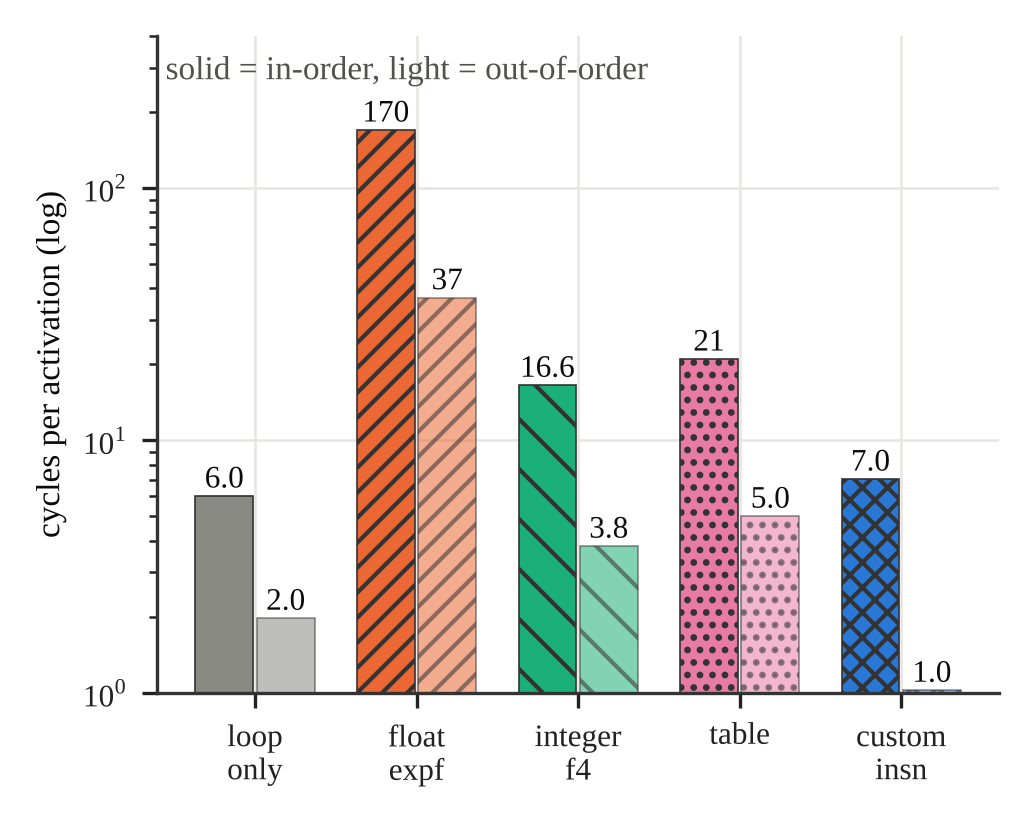
\includegraphics[width=\columnwidth]{fig1_cycles_per_activation.png}
\caption{Cycles per activation for the five variants on both cores (100 MHz, sorted inputs; logarithmic axis). Dark bars: in-order; light bars: out-of-order.}
\label{fig:cycles}
\end{figure}

Speedups of the instruction are 24.1$\times$ over \texttt{expf}, 2.35$\times$ over integer $f_4$ and 3.0$\times$ over the table in-order; 35.9$\times$, 3.72$\times$ and 4.9$\times$ out-of-order.  These are loop-level figures; the weakest baseline (\texttt{expf}) dominates them and they should not be read as system speedups. CPI \emph{falls} on the out-of-order core (0.17 for the instruction) but CPI alone misleads: the instruction raises CPI in-order relative to the table (1.17 vs 1.00) while still being 3$\times$ faster, because it removes instructions. The iron law must be read with all three terms.

\subsection{Latency, clock and pipelining (E2, E2b)}
\begin{figure*}[!t]
\centering
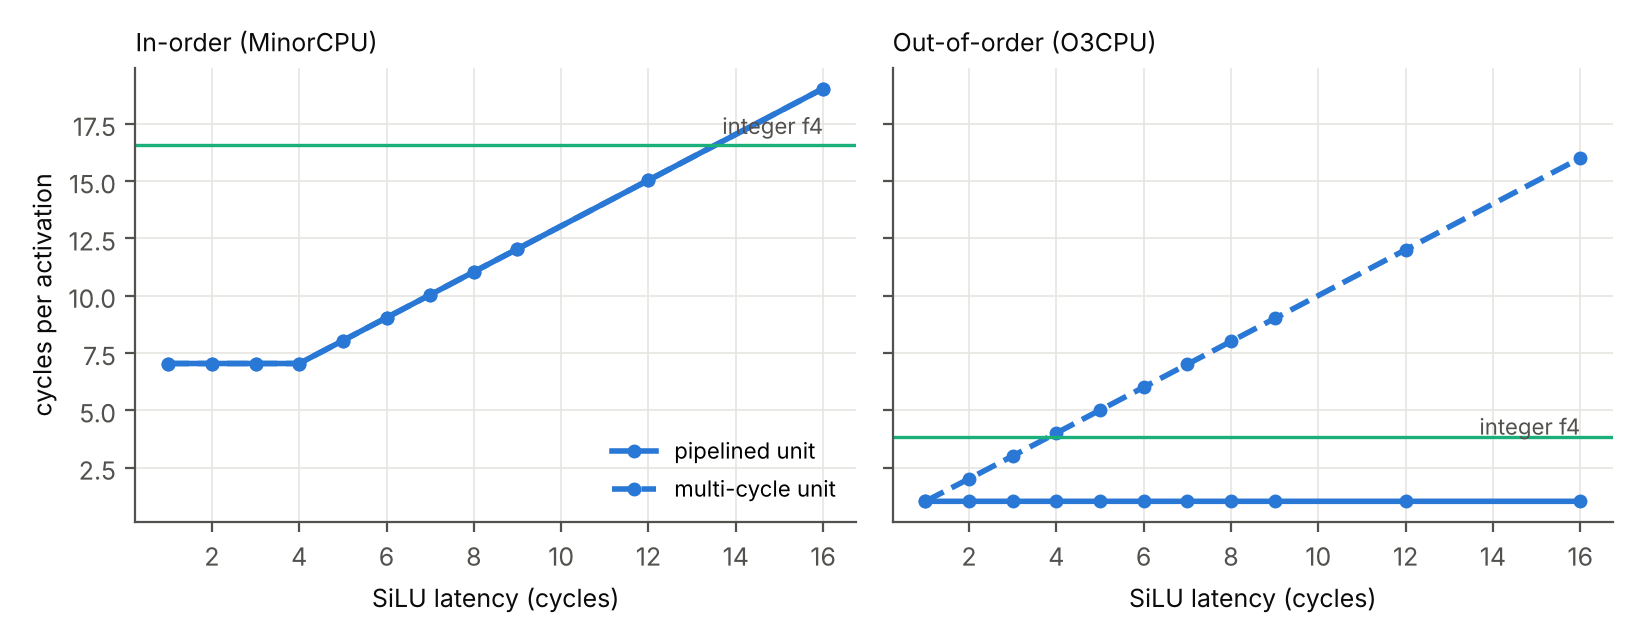
\includegraphics[width=0.98\textwidth]{fig2_latency_sweep.png}
\caption{Cycles per activation against custom-instruction latency (1 GHz core; instruction loop only).}
\label{fig:lat}
\end{figure*}
Fig.~\ref{fig:lat} varies latency from 1 to 16 cycles. In-order, cycles are flat up to latency 4 (the first few cycles are absorbed by the remaining loop instructions) and then grow one-for-one with latency; pipelined and unpipelined units give identical values, since an in-order core does not issue the next SiLU before the previous result is consumed. Out-of-order, a \emph{pipelined} unit hides every latency tested (1.03 cycles at 16), while an \emph{unpipelined} unit exposes it completely: 5 cycles at 500 MHz and 9 at 1 GHz. At 500 MHz an unpipelined unit is therefore \emph{slower} than integer $f_4$ (0.76$\times$ of its speed); at 1 GHz it is slower (0.42$\times$). This is a structural hazard in the textbook sense, and it implies that the 8.058 ns unit must be pipelined to be useful in a fast out-of-order core.

\begin{figure*}[!t]
\centering
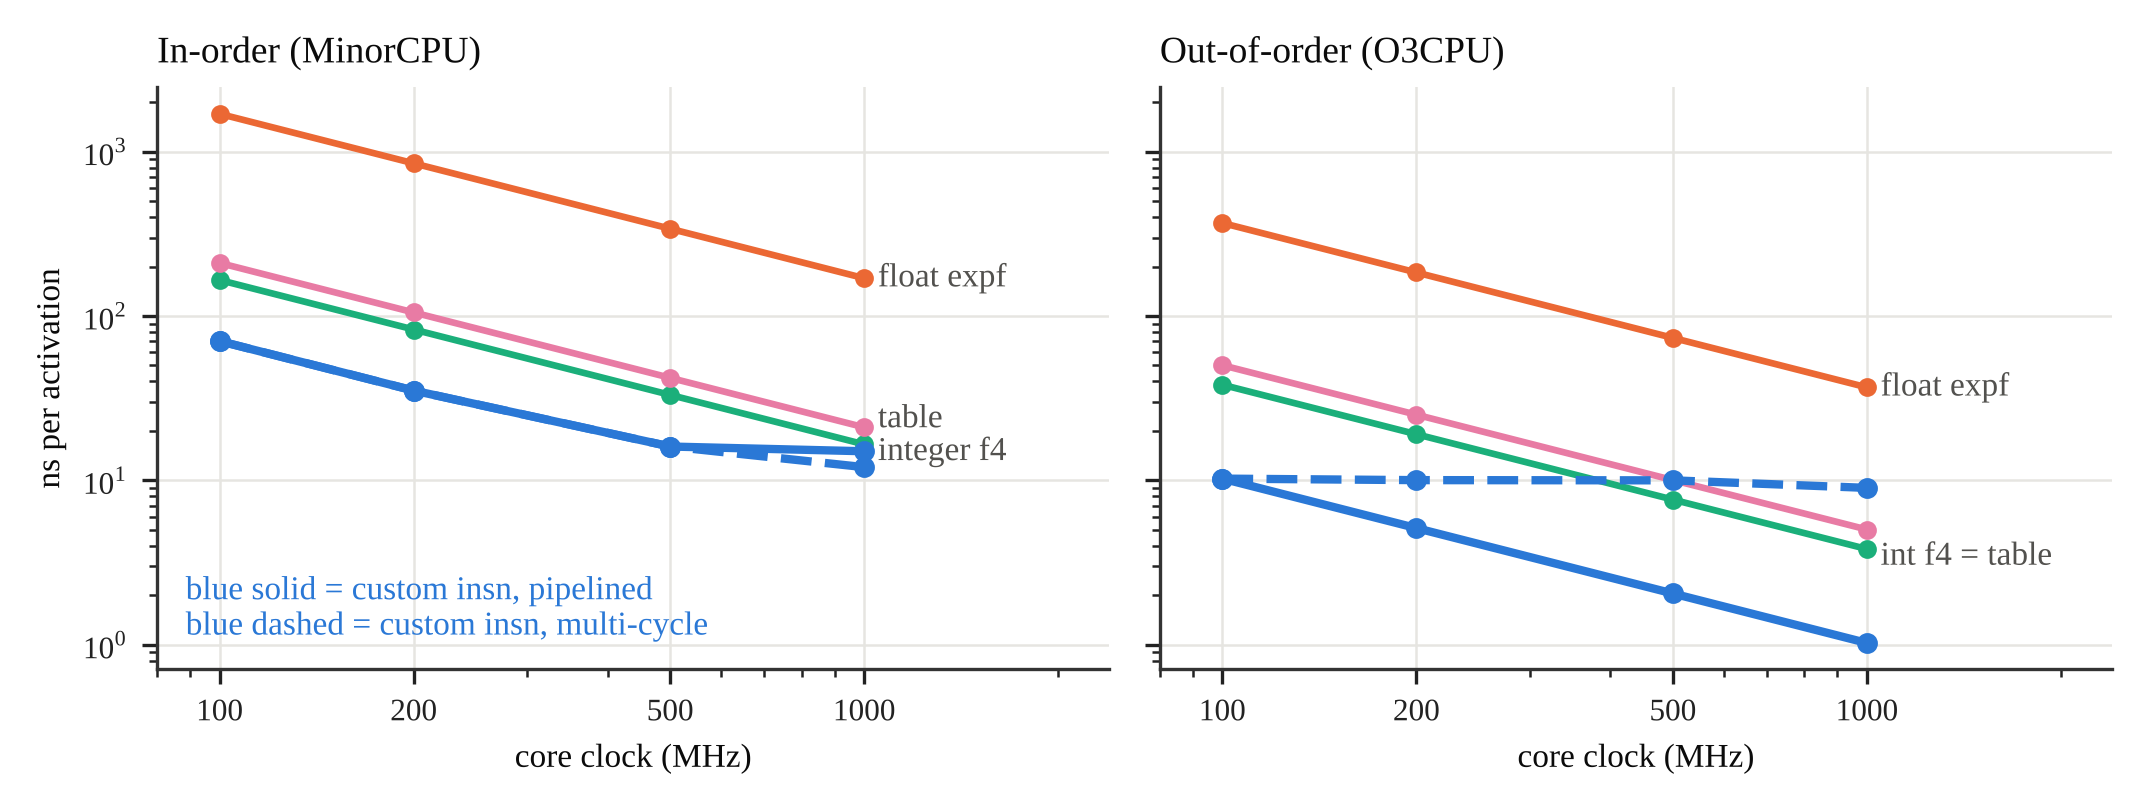
\includegraphics[width=0.98\textwidth]{fig3_time_vs_clock.png}
\caption{Wall-clock time per activation against core clock, for each core and each style of SiLU unit.}
\label{fig:clock}
\end{figure*}
Fig.~\ref{fig:clock} converts to time. Faster clocks raise the latency in cycles, so at 1 GHz the in-order core is only 1.1$\times$ (12-stage pipelined unit) to 1.4$\times$ (9-cycle multi-cycle unit) faster than integer $f_4$. Clocks above $\approx$123 MHz extrapolate an FPGA delay to faster logic and are illustrative only.

\subsection{Branch prediction (E4)}
\begin{figure*}[!t]
\centering
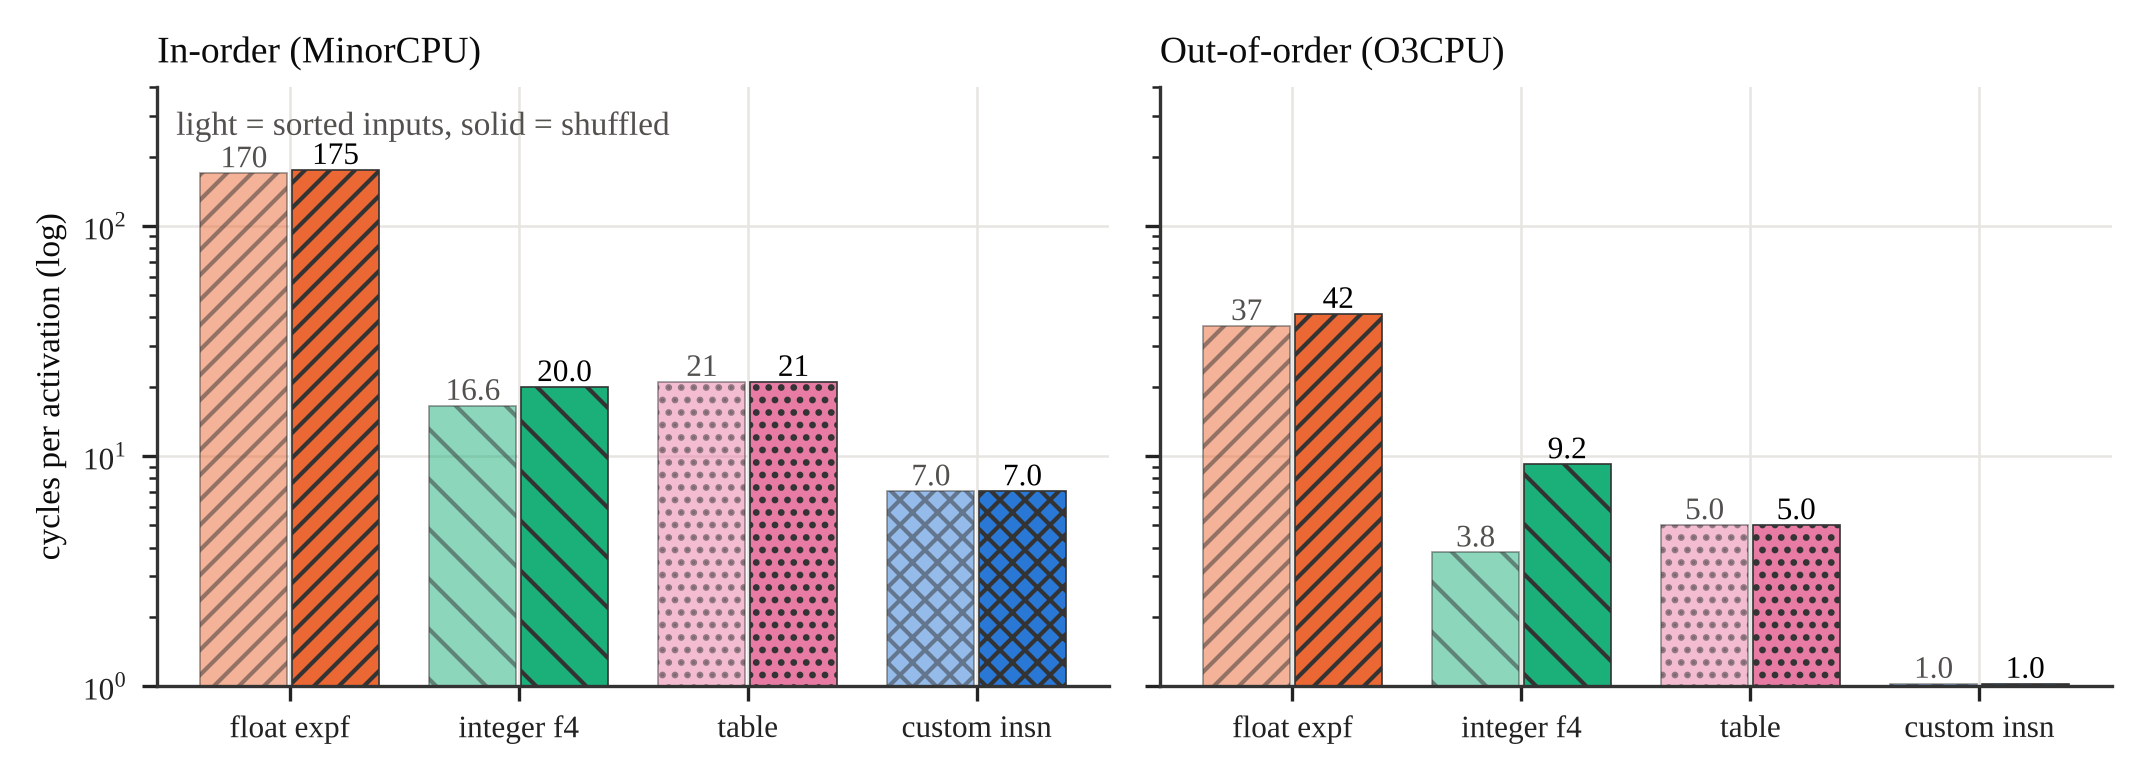
\includegraphics[width=0.98\textwidth]{fig6_branch_sorted_vs_shuffled.png}
\caption{Cycles per activation with sorted (light) and shuffled (dark) inputs at 100 MHz.}
\label{fig:branch}
\end{figure*}
Software $f_4$ is a compare chain. With sorted inputs the branches are perfectly predictable (0.005 mispredicts per activation), which flatters the software baseline. With shuffled inputs (a fixed xorshift permutation) it mispredicts 0.41 branches per activation (32 per 1000 instructions), costing +3.4 cycles in-order (16.6$\to$20.0) and +5.4 out-of-order (3.8$\to$9.2). \texttt{expf} adds 0.44 mispredicts per activation (+5.7 and +4.8 cycles). The table and the custom instruction have no data-dependent branch and are unaffected (Fig.~\ref{fig:branch}). Against shuffled inputs, the instruction is 2.8$\times$ (in-order) and 9.0$\times$ (out-of-order) faster than integer $f_4$; the order-of-magnitude advantage of the out-of-order result comes in large part from removing branch mispredictions.

\subsection{Code-placement sensitivity (E7)}
Tiny loops in gem5 are front-end sensitive. Compiling the same source with different loop alignments moves the out-of-order instruction loop between 1.03 and 4.02 cycles per activation and integer $f_4$ between 3.82 and 5.69 (Table~\ref{tab:align}); inside the convolution layer the extra cost of an activation varies by more than 10 cycles. This is an artefact of the simulated front end, not of the instruction, and sets the resolution of this study: differences of $\pm$1--3 cycles per activation between the cheap variants are not conclusions. Only \texttt{expf} is cleanly separated in the conv layer.

\begin{table}[t]
\caption{Loop Alignment Sensitivity (Cycles per Activation, 100 MHz, Minimum--Maximum over Five Alignments)}
\label{tab:align}
\centering\small
\begin{tabular}{lcc}
\toprule
Variant & In-order & Out-of-order\\
\midrule
float \texttt{expf} & 169.8--169.8 & 36.6--36.9\\
integer $f_4$ & 16.6--18.1 & 3.8--5.7\\
table & 20.0--21.0 & 5.0--6.0\\
custom insn & 7.0--9.0 & 1.0--4.0\\
\bottomrule
\end{tabular}
\end{table}

\subsection{Cache pressure (E6)}
\begin{table}[t]
\caption{Cycles per Activation versus L1 Data-Cache Size (500 MHz, Shuffled Inputs, No L2 Cache)}
\label{tab:cache}
\centering\small
\begin{tabular}{llccccc}
\toprule
Core & Variant & 512 B & 1 kB & 2 kB & 4 kB & 64 kB\\
\midrule
In-order & integer $f_4$ & 20.25 & 20.26 & 20.01 & 19.98 & 19.98\\
 & table & 28.49 & 21.59 & 21.23 & 21.07 & 21.03\\
 & custom insn & 8.53 & 8.54 & 8.08 & 8.04 & 8.04\\
\midrule
Out-of-order & integer $f_4$ & 9.76 & 9.76 & 9.25 & 9.23 & 9.23\\
 & table & 6.08 & 5.20 & 5.12 & 5.03 & 5.02\\
 & custom insn & 1.48 & 1.48 & 1.06 & 1.03 & 1.03\\
\bottomrule
\end{tabular}
\end{table}
A table needs data memory; the instruction does not. Table~\ref{tab:cache} shows that shrinking the L1 data cache from 64 kB to 512 B (working set: 2 kB of inputs plus 0.5 kB of table) costs the table 35\% in-order (21.0$\to$28.5) and 21\% out-of-order (5.0$\to$6.1); the instruction moves from 8.0 to 8.5 and from 1.0 to 1.5 (its only loads are the inputs). Once the cache is 1 kB or larger the table loses at most 3\% in-order, so at this table size the instruction's advantage over the table is mostly the instruction count, not the cache. A bigger table would suffer sooner.

\subsection{Whole model: YOLOv8n and Amdahl's law (E5)}
\textbf{Accuracy.} Table~\ref{tab:acc} gives COCO128 accuracy. Most of the loss is fixed-point rounding itself ($-0.0066$ mAP50--95); $f_4$ adds about $0.0015$, well below the noise of a 128-image set. 8.8\% of YOLOv8n's activation inputs lie outside $[-4,4]$ (Fig.~\ref{fig:inputs}), the region where a segment-based approximation relies on its tail rules, so restricting evaluation to $[-4,4]$ ignores a non-trivial share of real inputs. The micro-benchmark sweeps $[-4,4)$, where the six segments are active; the model run exercises the tails as well.

\begin{table}[t]
\caption{YOLOv8n Accuracy on COCO128 (Relative Comparison Only; 57 of 57 SiLU Modules Replaced in Each Row)}
\label{tab:acc}
\centering\small
\begin{tabular}{lccc}
\toprule
Activation & mAP50 & mAP50--95 & $\Delta$\\
\midrule
exact SiLU & 0.6024 & 0.4439 & ---\\
exact, Q6.10 rounding & 0.5924 & 0.4374 & $-0.0066$\\
$f_4$ (16-bit strict) & 0.5991 & 0.4359 & $-0.0081$\\
$f_4$ (exact tails) & 0.6007 & 0.4359 & $-0.0080$\\
257-entry table & 0.5958 & 0.4373 & $-0.0066$\\
\bottomrule
\end{tabular}
\end{table}

\begin{figure}[t]
\centering
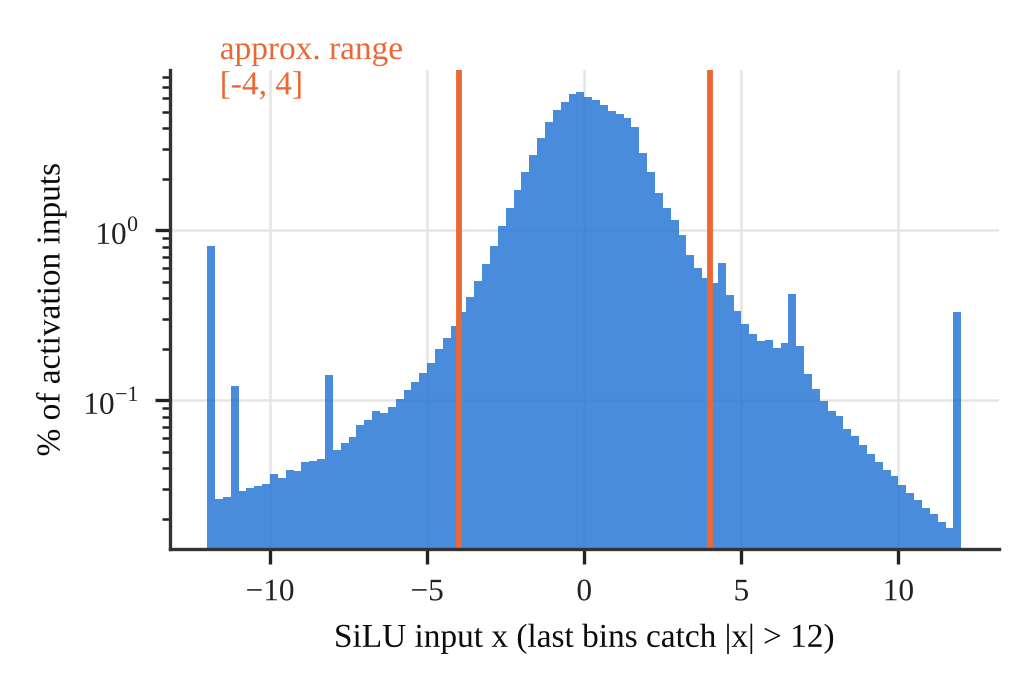
\includegraphics[width=\columnwidth]{fig5_yolo_activation_inputs.png}
\caption{Distribution of YOLOv8n activation inputs; the vertical lines mark $[-4,4]$, where the six segments are active.}
\label{fig:inputs}
\end{figure}

\textbf{Speed.} The convolution layer measures cycles per MAC (median over five alignments: 5.67 in-order, 1.15 out-of-order at 500 MHz); the shuffled-loop experiment gives cycles per activation. With 315 MACs per activation in YOLOv8n,
\begin{equation}
S=\frac{t_{MAC}/k+t_{act}^{base}}{t_{MAC}/k+t_{act}^{insn}}
\end{equation}
where $t_{MAC}$ and $t_{act}$ are the whole-network MAC and activation times (MACs $\times$ cycles per MAC; activations $\times$ cycles per activation) and $k$ is the speedup applied to the MAC part (SIMD, accelerator); this is Amdahl's law with the activation share $p=t_{act}^{base}/(t_{MAC}/k+t_{act}^{base})$. Fig.~\ref{fig:amdahl} and Table~\ref{tab:amdahl} give the estimate. On a scalar core the activation is 8.7\% (in-order) to 9.9\% (out-of-order) of run time with \texttt{expf} and under 2\% with integer $f_4$, so the custom instruction gives only 1.09--1.11$\times$ over \texttt{expf} and 1.01--1.02$\times$ over integer $f_4$. If MACs are 16$\times$ faster, the figures rise to 2.5--2.7$\times$ and 1.1--1.3$\times$. The instruction matters when the multiply-accumulate part is accelerated, not on a scalar core --- a direct, quantitative Amdahl result.

\begin{figure*}[!t]
\centering
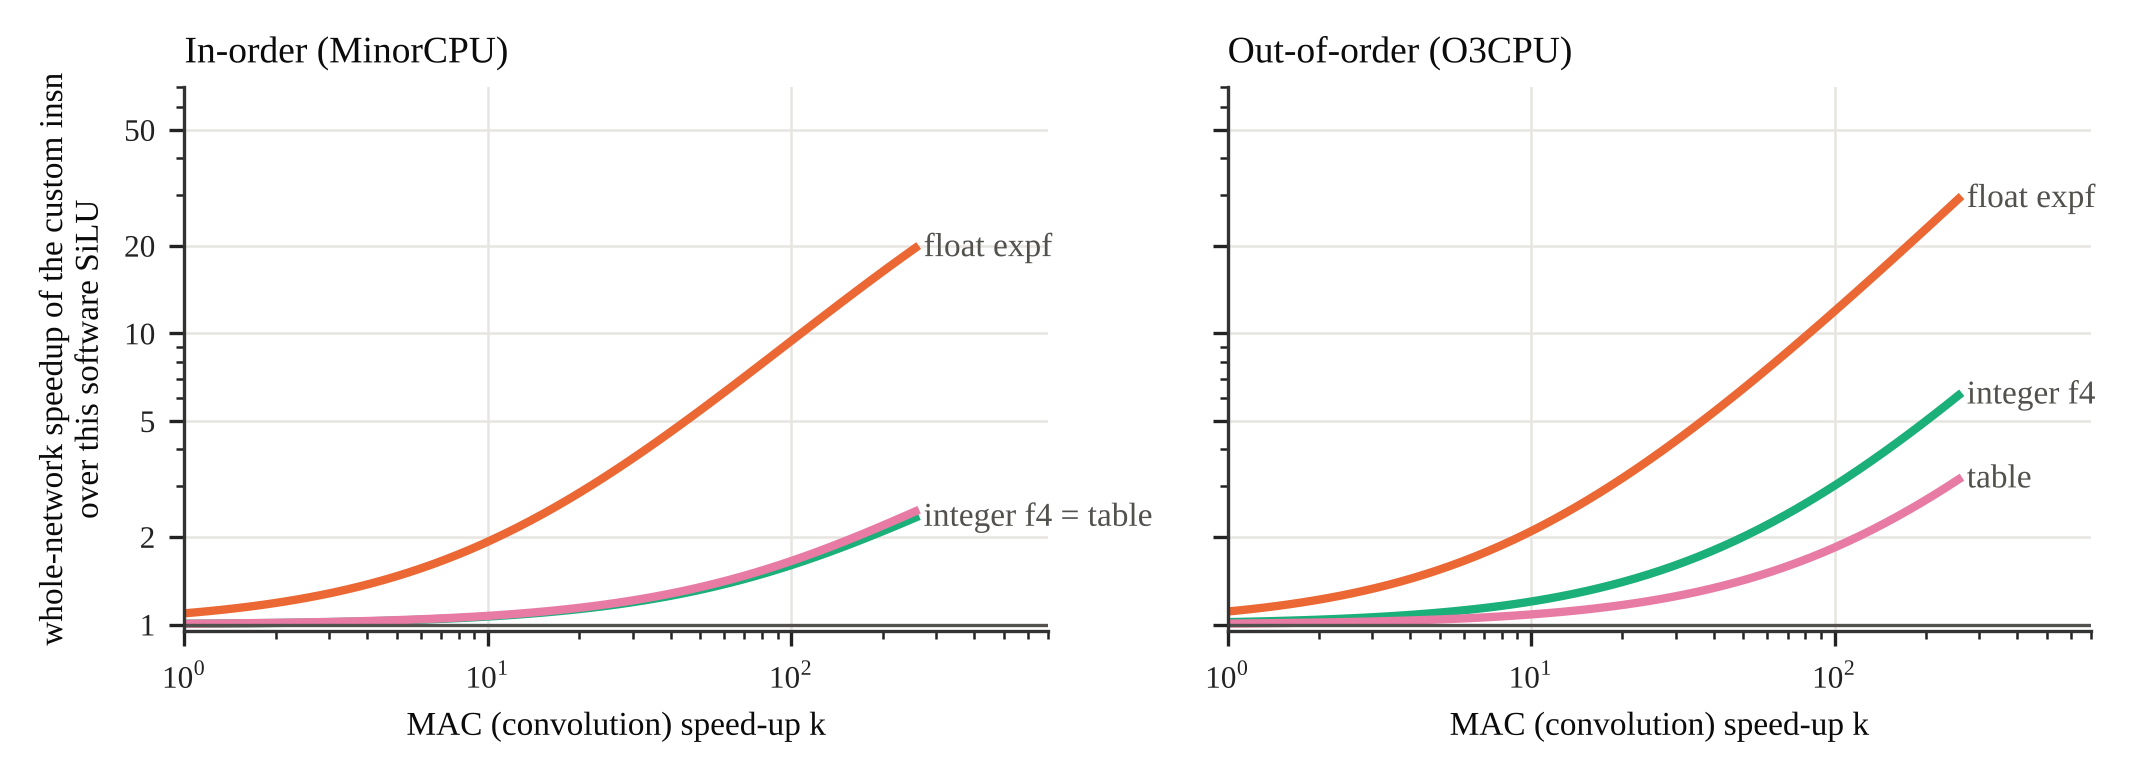
\includegraphics[width=0.98\textwidth]{fig4_amdahl_yolov8n.png}
\caption{Estimated whole-network speedup for YOLOv8n against the MAC speedup $k$ (500 MHz).}
\label{fig:amdahl}
\end{figure*}

\begin{table}[t]
\caption{Estimated Whole-Network Speedup of the Custom Instruction (YOLOv8n, 500 MHz)}
\label{tab:amdahl}
\centering\small
\begin{tabular}{lcccc}
\toprule
 & \multicolumn{2}{c}{vs \texttt{expf}} & \multicolumn{2}{c}{vs integer $f_4$}\\
$k$ & In-order & O3 & In-order & O3\\
\midrule
1 & 1.09 & 1.11 & 1.01 & 1.02\\
4 & 1.37 & 1.44 & 1.03 & 1.08\\
16 & 2.48 & 2.75 & 1.10 & 1.32\\
64 & 6.60 & 8.00 & 1.40 & 2.28\\
\bottomrule
\end{tabular}
\end{table}

\section{Discussion}
\textbf{What the instruction buys.} It replaces about 13 integer instructions and a compare chain by one operation. That is a large win against a library \texttt{expf} (24--36$\times$ on the loop) and a moderate one against well-written integer code (2.4--3.7$\times$, more with unpredictable data). The honest system-level statement is that a scalar RISC-V core running YOLOv8n gains about 10\% over \texttt{expf} and about 1--2\% over integer $f_4$; the instruction becomes valuable only in a balanced design in which the MACs are already accelerated.

\textbf{What the microarchitecture decides.} The same instruction is limited by dependence latency in order, by issue rate and unit pipelining out of order, and by branch behaviour in its software competitor. The iron-law terms move in different directions with the core: IC always falls, CPI falls or rises, and $T_{clk}$ is set by the unit's pipeline depth. Because the out-of-order core overlaps iterations, a pipelined unit makes latency nearly irrelevant, whereas a unit that cannot accept one operation per cycle destroys the benefit.

\textbf{Accuracy cost.} $f_4$ is a coarse approximation (mean error 0.028, about 60$\times$ the table's) but its effect on detection accuracy beyond Q6.10 rounding is within the noise of our test set. This does not prove equivalence on the full COCO validation set.

\section{Threats to Validity}
\begin{itemize}
\item One activation loop and one scalar convolution layer; the network-level numbers are a scaled estimate, not a simulation of YOLOv8n.
\item Alignment sensitivity of $\pm$1--3 cycles (Table~\ref{tab:align}); the cheap variants cannot be ranked inside the conv layer.
\item The 8.058 ns delay is from a slow-corner FPGA; 0.3 ns per pipeline stage is an assumption; no clock uncertainty was in the timing constraints; clocks above 123 MHz are extrapolations.
\item Default in-order and out-of-order gem5 models, one SiLU unit, no L2 in E6; compiler is clang with musl \texttt{expf}, not GCC with glibc, which would change the \texttt{expf} baseline.
\item COCO128 is a small subset of train2017, used only for comparing activations.
\item No power or area comparison with a floating-point SiLU unit.
\item Not done: GPU comparison (e.g.\ Vortex) and a full-system run of YOLOv8n in gem5.
\end{itemize}

\section{Conclusion}
A multiplier-free SiLU instruction is a 24--36$\times$ win on the activation loop against \texttt{expf} and a 2.4--3.7$\times$ win against integer C, but a 1.1$\times$ and 1.01--1.02$\times$ win respectively on a scalar-core YOLOv8n; its value grows with how much the rest of the network is accelerated. It must be pipelined to help an out-of-order core, and its advantage over software is larger for unpredictable data because it removes branches. The flow that derives its latency from synthesis is scripted and reproducible, with all raw runs, tables and figures kept in the project repository.

\section{Artifact Availability}
All numbers are produced by commands in \texttt{docs/REPRODUCE.md}; raw gem5 outputs are in \texttt{results/raw/} and the tables and figures in this report are generated from them by \texttt{scripts/make\_results.py}. 296 gem5 runs were made.

\begin{thebibliography}{10}
\bibitem{elfwing2018} S.~Elfwing, E.~Uchibe, and K.~Doya, ``Sigmoid-weighted linear units for neural network function approximation in reinforcement learning,'' \emph{Neural Netw.}, vol.~107, pp.~3--11, 2018.
\bibitem{ramachandran2017} P.~Ramachandran, B.~Zoph, and Q.~V.~Le, ``Searching for activation functions,'' 2017, arXiv:1710.05941.
\bibitem{spagnolo2025} F.~Spagnolo, S.~Perri, and P.~Corsonello, ``Approximate Swish activation function for low-energy yet low-error VLSI implementations,'' in \emph{Proc.\ IEEE Comput.\ Soc.\ Annu.\ Symp.\ VLSI (ISVLSI)}, 2025, doi: 10.1109/ISVLSI65124.2025.11130259.
\bibitem{hennessy} J.~L.~Hennessy and D.~A.~Patterson, \emph{Computer Architecture: A Quantitative Approach}, 6th~ed. Cambridge, MA, USA: Morgan Kaufmann, 2017.
\bibitem{amdahl1967} G.~M.~Amdahl, ``Validity of the single processor approach to achieving large scale computing capabilities,'' in \emph{Proc.\ AFIPS Spring Joint Comput.\ Conf.}, 1967, pp.~483--485.
\bibitem{binkert2011} N.~Binkert \emph{et al.}, ``The gem5 simulator,'' \emph{ACM SIGARCH Comput.\ Archit.\ News}, vol.~39, no.~2, pp.~1--7, May 2011.
\bibitem{lowepower2020} J.~Lowe-Power \emph{et al.}, ``The gem5 simulator: Version 20.0+,'' 2020, arXiv:2007.03152.
\bibitem{riscv} A.~Waterman and K.~Asanovi\'c, Eds., \emph{The RISC-V Instruction Set Manual, Volume I: Unprivileged ISA}, Document Version 20191213, RISC-V International, Dec. 2019.
\bibitem{ultralytics} G.~Jocher, A.~Chaurasia, and J.~Qiu, ``Ultralytics YOLOv8,'' 2023. [Online]. Available: https://github.com/ultralytics/ultralytics
\end{thebibliography}

\end{document}
